%!TEX root = ../main.tex

\begin{frame}{Tarefa de Aprendizado}
  \vskip2\baselineskip
	\begin{itemize}
	\item Problema abordado como uma \alert{tarefa de classificação binária}
	\item \alert{Entrada:}
	\begin{itemize}
		\item Imagem em escala de cinza com dimensões de $256 \times 256$ \emph{pixels} contendo duas assinaturas manuscritas (uma de referência e outra para a inferência)
	\end{itemize}
	\item \alert{Saída:}
	\begin{itemize}
		\item Classificação da assinatura quanto à sua autenticidade (autêntica ou forjada)
	\end{itemize}
	\end{itemize}

	\begin{figure}
		\caption{Visão geral da tarefa de aprendizado considerada}
		\label{fig:esquema-solucao}
		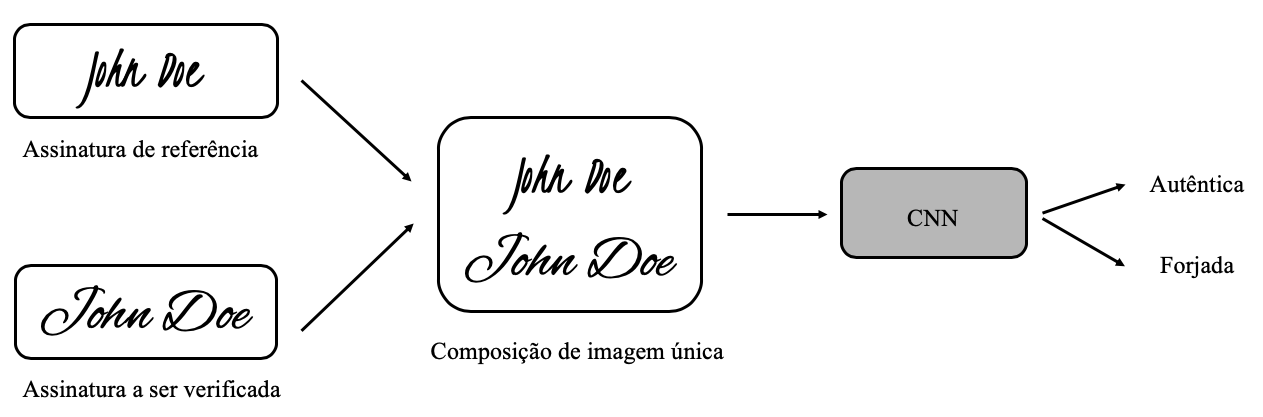
\includegraphics[width=0.5\textwidth]{img/esquema-solucao}
	\end{figure}
\end{frame}

\begin{frame}{Tarefa de Aprendizado}

\begin{itemize}
  \item Partição dos exemplos utilizando o método \emph{holdout}
    \begin{itemize}
      \item $70\%$ para treinamento;
      \item $10\%$ para validação;
      \item $20\%$ para teste.
    \end{itemize}
  \bigskip
  \item Utilização das métricas Acurácia e \emph{F-score} para análise de desempenho dos modelos
\end{itemize}

\end{frame}

\begin{frame}{Coleta do conjunto de Dados}
  \vskip2\baselineskip
  \begin{itemize}
    \item \emph{Signature Verification Competition} 2009 (SigComp2009)
    \item Dois conjuntos de dados foram utilizados na competição:
    \begin{itemize}
      \item \emph{Norwegian Information Security Donders Centre for Cognition} (NISDCC)
      \item \emph{Netherlands Forensic Institute} (NFI)
    \end{itemize}
    \item Informações \emph{online} e \emph{offline} das assinaturas
  \end{itemize}

  \begin{table}[h!]
\centering
\caption{Quantitativo de indivíduos e assinaturas \emph{offline} por conjunto de dados.}
\label{tab:demonstracao-dataset}
\resizebox{\textwidth}{!}{
\begin{tabular}{c C{2cm} C{2cm} C{3.25cm} C{2.5cm} C{2.5cm} C{2.25cm}}
  \toprule
   \textbf{Conjunto}& \textbf{Autores originais} & \textbf{Autores forjadores} & \textbf{Autores originais com assinaturas forjadas} & \textbf{Assinaturas genuínas}  & \textbf{Assinaturas forjadas} & \textbf{Total de assinaturas} \\
  \midrule
  NISDCC & 12 & 31 & 12 & 60 & 1.838 & 1.898 \\
  NFI & 79 & 33 & 19 & 940 & 624 & 1.564 \\
  \bottomrule
\end{tabular}}
\end{table}
\end{frame}

\begin{frame}{Preparação dos Dados}
  \vskip2\baselineskip
  \begin{itemize}
    \item Combinação e redimensionamento das imagens
    \bigskip
    \item Separação dos exemplos \alert{autênticos} conforme o método \emph{holdout}
    \item Exemplos \alert{forjados} necessitaram de um diferente tipo de separação
  \end{itemize}

  \begin{table}[h!]
	\centering
	\caption{Quantitativo de exemplos.}
	\label{tab:divisao-dados}
	\resizebox{!}{1.5cm}{\begin{tabular}{c c c c}
		\toprule
		\textbf{Conjunto} & \textbf{Tipo de Exemplo} & \textbf{Quantidade de Dados} & \textbf{Proporção}\\
		\midrule
		\multirow{2}{*}{Treinamento} & Autêntico & 9.374 & $54\%$ \\
    & Forjado & 8.131 & $46\%$\\
     \midrule
		 \multirow{2}{*}{Validação} & Autêntico & 947 & $46\%$ \\
     & Forjado & 1.134 & $54\%$\\
		 \midrule
		 \multirow{2}{*}{Teste} & Autêntico & 2.257 & $27\%$ \\
     & Forjado & 6.119 & $73\%$\\
		\bottomrule
	\end{tabular}}
  \end{table}
\end{frame}


\begin{frame}{Preparação dos Dados}
  \begin{figure}[h!]
  \centering
  \caption{Representação gráfica da proporção dos exemplos por classe e finalidade na tarefa de aprendizado considerada.}
  \label{fig:divisao-dados}
  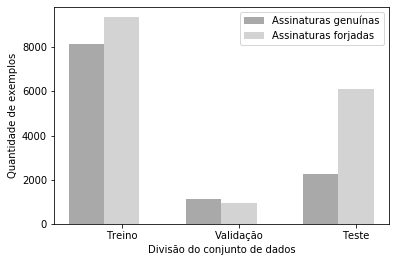
\includegraphics[width=0.3\textwidth]{./img/divisao-dados}
  \end{figure}

  \begin{itemize}
    \item Normalização dos \emph{pixels} das imagens ao serem fornecidas às CNNs
  \end{itemize}
\end{frame}

\begin{frame}{\Large{Modelos, Parâmetros e Hiperparâmetros Utilizados}}
\begin{itemize}
  \item Arquiteturas de CNNs escolhidas: LeNet, AlexNet, MobileNet, SqueezeNet, VGG-16 e Inception
\end{itemize}

\begin{table}[h!]
	\centering
	\caption{Valores dos hiperparâmetros selecionados para a elaboração dos modelos.}
	\label{tab:parametros}
  \resizebox{!}{0.8cm}{
	\begin{tabular}{c c C{3cm} C{3cm}}
		\toprule
		 \textbf{Épocas} & \textbf{\emph{Patience}} & \textbf{Otimizador} & \textbf{Função de ativação}  \\
		\midrule
		200 & 5, 10 e 15 & SGD, Adam e RMSprop & ReLU, ELU, SELU e Leaky ReLU \\
		\bottomrule
	\end{tabular}}
\end{table}

\begin{itemize}
  \item Busca em \emph{grid} nos hiperparâmetros quando possível
  \item Demais casos, hiperparâmetros típicos
\end{itemize}

\end{frame}
